\section{Introduction}

Networks encompass a diverse range of physical media, topologies, and protocols. 
To effectively manage this complexity, a layered approach is crucial.
\begin{figure}[H]
    \centering
    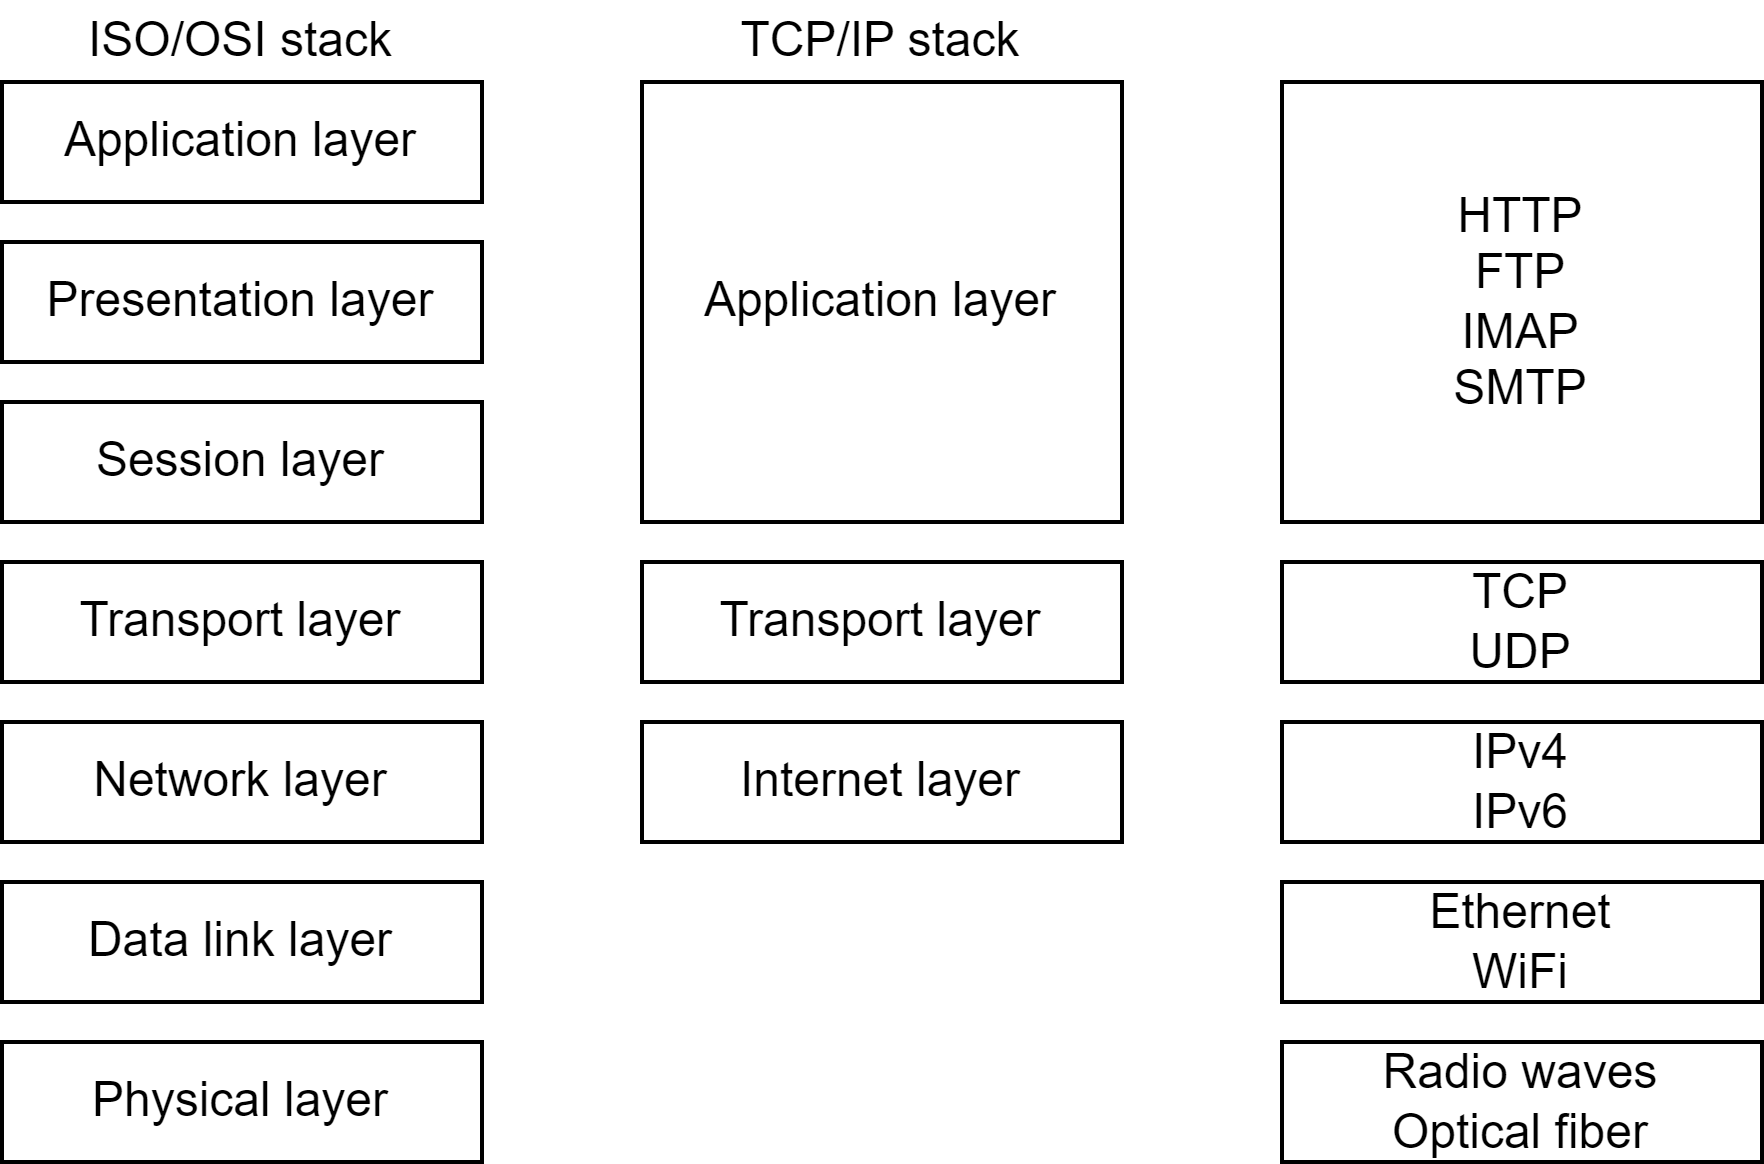
\includegraphics[width=0.75\linewidth]{images/lp.png}
    \caption{Layering and protocols}
\end{figure}

In network communications, hosts are uniquely identified by addresses, similar to phone numbers or postal addresses. 
Each layer in the network stack utilizes its own addressing scheme:
\begin{itemize}
    \item \textit{Data link layer}: utilizes MAC addresses (for Ethernet), which are globally unique identifiers embedded in the Network Interface Card (NIC). 
        The Address Resolution Protocol (ARP) is used to map an IP address to a MAC address.
    \item \textit{Internet layer}: employs IP addresses to identify network hosts globally. 
        It includes both public and private addresses, with private addresses defined by RFC 1918 for IPv4.
    \item \textit{Transport layer}: uses port numbers to identify specific services on a host.
\end{itemize}

\paragraph*{Transport protocols}
Transport protocols facilitate communication between hosts:
\begin{itemize}
    \item \textit{User Datagram Protocol} (UDP): a connectionless protocol that provides a lightweight wrapper around an IP packet, primarily adding a port number for addressing.
    \item \textit{Transmission Control Protocol} (TCP): a connection-oriented protocol that manages state through concepts such as closed, open, and established connections. 
        It uses a three-way handshake to establish connections.
\end{itemize}

\begin{definition}[\textit{Denial Of Service}]
    A Denial of Service (DoS) attack targets the availability of a service, rendering it inaccessible to legitimate users.
\end{definition}
\begin{definition}[\textit{Sniffing}]
    Sniffing refers to the unauthorized reading of network packets, compromising confidentiality.
\end{definition}
\begin{definition}[\textit{Spoofing}]
    Spoofing involves forging network packets, thereby compromising the integrity and authenticity of communications.
\end{definition}